\documentclass[10pt, a5paper]{article}
\usepackage{pdfpages}
\usepackage{parallel}
\usepackage[T2A]{fontenc}
\usepackage{ucs}
\usepackage[utf8x]{inputenc}
\usepackage[polish,english,russian]{babel}
\usepackage{hyperref}
\usepackage{rotating}
\usepackage[inner=2cm,top=1.8cm,outer=2cm,bottom=2.3cm,nohead]{geometry}
\usepackage{listings}
\usepackage{graphicx}
\usepackage{wrapfig}
\usepackage{longtable}
\usepackage{indentfirst}
\usepackage{array}
\newcolumntype{P}[1]{>{\raggedright\arraybackslash}p{#1}}
\frenchspacing
\usepackage{fixltx2e} %text sub- and superscripts
\usepackage{icomma} % коскі ў матэматычным рэжыме
\PreloadUnicodePage{4}

\newcommand{\longpage}{\enlargethispage{\baselineskip}}
\newcommand{\shortpage}{\enlargethispage{-\baselineskip}}

\def\switchlang#1{\expandafter\csname switchlang#1\endcsname}
\def\switchlangbe{
\let\saverefname=\refname%
\def\refname{Літаратура}%
\def\figurename{Іл.}%
}
\def\switchlangen{
\let\saverefname=\refname%
\def\refname{References}%
\def\figurename{Fig.}%
}
\def\switchlangru{
\let\saverefname=\refname%
\let\savefigurename=\figurename%
\def\refname{Литература}%
\def\figurename{Рис.}%
}

\hyphenation{admi-ni-stra-tive}
\hyphenation{ex-pe-ri-ence}
\hyphenation{fle-xi-bi-li-ty}
\hyphenation{Py-thon}
\hyphenation{ma-the-ma-ti-cal}
\hyphenation{re-ported}
\hyphenation{imp-le-menta-tions}
\hyphenation{pro-vides}
\hyphenation{en-gi-neering}
\hyphenation{com-pa-ti-bi-li-ty}
\hyphenation{im-pos-sible}
\hyphenation{desk-top}
\hyphenation{elec-tro-nic}
\hyphenation{com-pa-ny}
\hyphenation{de-ve-lop-ment}
\hyphenation{de-ve-loping}
\hyphenation{de-ve-lop}
\hyphenation{da-ta-ba-se}
\hyphenation{plat-forms}
\hyphenation{or-ga-ni-za-tion}
\hyphenation{pro-gramming}
\hyphenation{in-stru-ments}
\hyphenation{Li-nux}
\hyphenation{sour-ce}
\hyphenation{en-vi-ron-ment}
\hyphenation{Te-le-pathy}
\hyphenation{Li-nux-ov-ka}
\hyphenation{Open-BSD}
\hyphenation{Free-BSD}
\hyphenation{men-ti-on-ed}
\hyphenation{app-li-ca-tion}

\def\progref!#1!{\texttt{#1}}
\renewcommand{\arraystretch}{2} %Іначай формулы ў матрыцы зліпаюцца з лініямі
\usepackage{array}

\def\interview #1 (#2), #3, #4, #5\par{

\section[#1, #3, #4]{#1 -- #3, #4}
\def\qname{LVEE}
\def\aname{#1}
\def\q ##1\par{{\noindent \bf \qname: ##1 }\par}
\def\a{{\noindent \bf \aname: } \def\qname{L}\def\aname{#2}}
}

\def\interview* #1 (#2), #3, #4, #5\par{

\section*{#1\\{\small\rm #3, #4. #5}}

\def\qname{LVEE}
\def\aname{#1}
\def\q ##1\par{{\noindent \bf \qname: ##1 }\par}
\def\a{{\noindent \bf \aname: } \def\qname{L}\def\aname{#2}}
}

\begin{document}
\title{Кратко о SO\_BUSY\_POLL}
\author{Евгений Рыбак, Минск, Беларусь\footnote{\url{engler@tut.by}, \url{http://lvee.org/en/abstracts/156}}}
\maketitle
\begin{abstract}
Performance of Linux network stack was always kept in mind during any implementation. Increasing demand for cloud services, multimedia content, high performance computing forces to search new ways of optimization. SO\_BUSY\_POLL is one of the way to improve processing of incoming network messages without changing source code of the product.
\end{abstract}
\subsubsection*{Введение}

Оптимизация скорости обработки входящих пакетов всегда была одной из главных задач сетевого стека. Рост облачных сервисов, объемов мультимедийного контента, высокопроизводительных систем (HPC) заставляет выискивать новые резервы для оптимизаций. SO\_BUSY\_POLL является еще одним способом улучшить производительность системы, практически не меняя исходный текст продукта.

\subsubsection*{Уровни стека TCP/IP}

Как известно, стек TCP/IP состоит из уровней, каждый из которых решает четко поставленную задачу.


\begin{figure}[h!]
  \centering 
  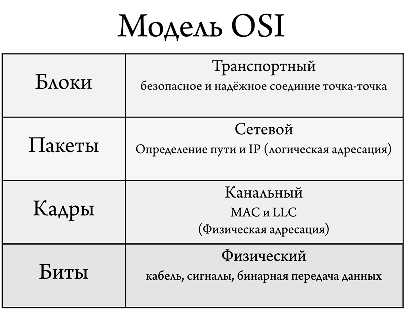
\includegraphics[scale=0.6]{15_2015_Osi-model-50}
\end{figure}


Физический уровень отвечает за передачу и прием электрических данных по сетевому кабелю, в соответствии с методами кодирования.

Канальный уровень отвечает за преобразование из электрического сигнала в цифровой кадр, аппаратную адресацию (MAC"=адрес).

Сетевой уровень отвечает за связывание отдельных подсетей, в целую сеть. Идентификация узла в сети осуществляется с помощью IP"=адреса.

Транспортный уровень отвечает за идентификацию процесса, в рамках узла, которому необходимо передать данные. Идентификация процесса осуществляется с помощью номера порта.

\subsubsection*{Методы обработки входящих пакетов}

Классически, есть два основных подхода для того, что бы узнать, что на сетевой адаптер пришли новые пакеты:

\begin{itemize}
  \item метод прерываний (IRQ);
  \item метод опроса (polling).
\end{itemize}

Каждый из методов имеет свои достоинства и недостатки: метод прерываний хорошо себя показал для небольшого объема трафика, когда прерывания генерируются не часто, не мешая процессору выполнять свои задачи. В случае большого и очень большого объема трафика метод является не очень эффективным; именно в этом случае метод опроса устройства является наиболее подходящим. Busy Poll (новая опция SO\_BUSY\_POLL) является усовершенствованием классического метода опроса, который уменьшает задержку (Latency) и увеличивает пропускную способность (Throughput).

\subsubsection*{Обзор опции SO\_BUSY\_POLL}

Начиная с версии ядра 3.11, ядро осуществляет поддержку опции сокета SO\_BUSY\_POLL.
В эко"=системе SO\_BUSY\_POLL \linebreak участвуют следующие компоненты:

\begin{itemize}
  \item ядро операционной системы;
  \item драйвер сетевой карты;
  \item настройки системы.
\end{itemize}

\textit{Поддержка ядра операционной системы}

Ядро должно быть собрано с опцией \linebreak CONFIG\_NET\_RX\_BUSY\_POLL.

\textit{Драйвер сетевой карты}

Драйвер сетевой карты должен реализовать обработчик функции, который отвечает за busy polling.

\textit{Настройки системы}

В сетевых настройках появились две новые опции: busy\_read, busy\_poll.
Значением является количество микросекунд, в течении которого ядро будет опрашивать входящую очередь сетевой карты (Ethernet RX queue).
Прочитать и записать значения можно следующим образом:

\begin{verbatim}
sysctl net.core.busy_read 
sysctl net.core.busy_poll
sysctl net.core.busy_read=50
sysctl net.core.busy_poll=50
\end{verbatim}

Также рассмотрим влияние опции SO\_BUSY\_POLL на различные методы чтения TCP/UDP"=сокетов.

\subsubsection*{Отличие busy poll от NAPI poll}

\begin{figure}[h!]
  \centering 
  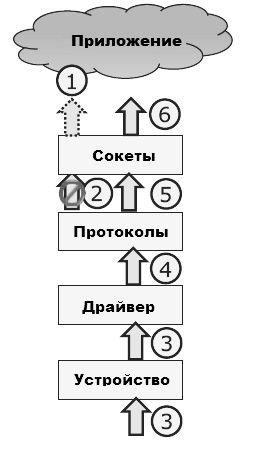
\includegraphics[scale=0.6]{15_2015_classic-packet-path-wo-busy-poll-ru}
\end{figure}

На рисунке выше показана работа приложения с точки зрения \linebreak NAPI poll. Схема включает следующие этапы:

\begin{enumerate}
  \item Приложение создает сокет и пытается из него прочитать данные.
  \item Данные отсутствуют, ожидаем момент, когда они появятся в буфере сокета.
  \item Данные приходят на интерфейс.
  \item Генерируется прерывание, данные передаются на уровень протоколов.
  \item Данные передаются в буфер сокета.
  \item Приложение может прочитать данные из сокета.
\end{enumerate}

В отличие от предыдущей, схема работы с включенной опцией SO\_BUSY\_POLL выглядит так:

\begin{figure}[h!]
  \centering 
  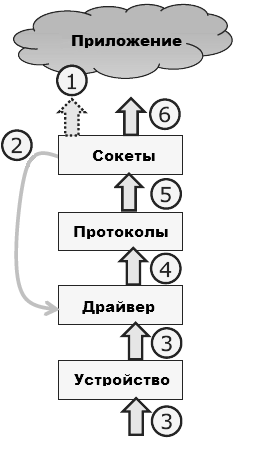
\includegraphics[scale=0.6]{15_2015_classic-packet-path-with-busy-poll-ru}
\end{figure}


\begin{enumerate}
  \item Приложение создает сокет и пытается из него прочитать данные.
  \item Если данных в буфере сокета нету, переходим к функции драйвера busy poll.
  \item Данные приходят на интерфейс.
  \item Генерируется прерывание, данные передаются на уровень протоколов.
  \item Данные передаются в буфер сокета.
  \item Приложение может прочитать данные из сокета.
\end{enumerate}

Одна из отличительных возможностей busy poll заключается в том, что если данные в буфере сокета отсутствуют, то нам не надо ждать прерывания от драйвера сетевой карты, как в случае с NAPI poll. Busy poll инициирует «принудительную» передачу пакетов из входящей очереди драйвера в очередь сокета, тем самым исключая «лишнее» переключение контекста и прерывание.

Еще одним моментом, на который стоит обратить внимание, является то, что в случае обработчика NAPI poll система передает количество пакетов, которое она готова обработать в данный момент. Если количество пакетов в очереди драйвера больше, чем количество пакетов, которое система готова обработать в текущий момент, то обработчик NAPI poll будет еще раз поставлен в очередь вызовов; через некоторый промежуток времени обработчик будет вызван в очередной раз.

В случае с busy poll, обработчик busy polling будет вызываться в течении времени, которое будет указано в опции SO\_BUSY\_POLL или настройках busy\_\{read,poll\}

\subsubsection*{Источники}

\begin{thebibliography}{9}
  \bibitem{sdf1} {A way towards Lower Latency and Jitter.} \url{http://www.linuxplumbersconf.org/2012/wp-content/uploads/2012/09/2012-lpc-Low-Latency-Sockets-slides-brandeburg.pdf}
  \bibitem{sdf2} {Open Source Kernel Enhancements for Low Latency Socket.} \url{http://www.intel.com/content/dam/www/public/us/en/documents/white-papers/open-source-kernel-enhancements-paper.pdf}
  \bibitem{sdf3} {Net: low latency Ethernet device polling.} \url{https://lwn.net/Articles/540281/}
  \bibitem{sdf4} {Understanding Linux Network Internals.} \url{http://www.amazon.com/Understanding-Network-Internals-Christian-Benvenuti/dp/0596002556}
  \bibitem{sdf5} {Linux Kernel Development.} \url{http://www.amazon.com/Linux-Kernel-Development-Robert-Love/dp/0672329468/ref=sr_1_1?s=books&ie=UTF8&qid=1434287714&sr=1-1&keywords=Linux.Kernel.Development}
  \bibitem{sdf6} {Linux Kernel Sources 3.18.14.} \url{https://www.kernel.org/pub/linux/kernel/v3.x/linux-3.18.14.tar.gz}
\end{thebibliography}
\end{document}
